% Load the base class
\documentclass[minted, draw, cover = contour]{../tex/hebdomon}
%    
\begin{document}
% 
%----------------------------------------------------------------------------------------------
\Title{Hebdomon Report and Documentation Standard}
\Institution{Management Center Innsbruck}
\SubTitle{v0.1.1 - Angry Avocado}
\StudentName{D. T. McGuiness}
\Email{dtm@mci4me.at}
\StudentNumber{21001}
\Semester{5}
\Degree{B.Sc}
\ModuleName{Robotic \& Vision}
\MakeTitle
%----------------------------------------------------------------------------------------------
\CopyRight
\StudentDeclaration
%----------------------------------------------------------------------------------------------

\tableofcontents
\newpage

\Chapter{The Hebdomon Template}
\Section{Introduction}

This document is designed to create an abstraction layer for the \LaTeX\, and \TeX\,
commands and MACROs to hide away the programming aspect (i.e., command declarations) and
ease into LaTeX programming as a means of introduction.

While some commands are have been changed \hlight{NO} command (or primitive) has been
overwritten so feel free to use the original ones if you wish.

\begin{warning}
	As to the best of the authors knowledge, the original commands should work
	but the aesthetics may be compromised.
\end{warning}

\Section{Title Formatting}

To begin a new content, always start the content with a chapter heading. To
insert the chapter with an additional \pcode{minitoc}
use \pcode{\Chapter} command, which produces an heading as
you see at the beginning of this page.
\\\\
To have a heading without a \pcode{minitoc} use the standard \pcode{\chapter}.

The document relies on the user to use the \hlight{correct} title commands to
keep the formatting consistent. The commands that starting with a
capital letter are the overloaded commands of the standard ones.
The following are the current ones in this version:
%
\begin{Code}{latex}{Types of Headers}
	\Chapter{...} % Allows entering chapters with mini table of contents
	\Section{...} % Allows section titles with blue tint
	\Subsection{...} % Allows subsection titles with blue tint
	\Subsubsection{...} % Allows subsubsection titles with blue tint
\end{Code}
%
\begin{warning}
	Unless there is a specific reason, it is suggested to use the aforementioned
	commands. However, original LaTeX command should work as well if you want to use.
\end{warning}

\Subsection{Page Geometry}

The page geometry is set to the following settings. This is done using the
standard package \pcode{\usepackage{geometry}} which is defined in the
\pcode{Hebdomon.cls}.
%
\begin{itemize}[leftmargin=!,labelindent=-29.2pt]
	\item[\textbf{top}] 2.5cm,
	\item[\textbf{right}] 2.0cm,
	\item[\textbf{bottom}] 2.5cm,
	\item[\textbf{left}] 3.0cm.
\end{itemize}
%
\Section{Image Positioning}
%
The image positioning could be done with the following code snippet:
%
\begin{Code}{latex}{A Figure Environment}
	\begin{figure}[ht]
		\centering
		\includegraphics[options]{path.pdf}
		\caption{}\label{fig:...}
	\end{figure}
\end{Code}
%
Here there are a few options worth mentioning:
% 
\begin{hgitemize}
	\item[\pcode{path.pdf}] The place where the image is kept. If the
	image is in the same folder where the \pcode{main.tex} file resides, it is as
	simple as writing the files name. If the file (i.e., \pcode{innsbruck.jpg}) is in a
	folder called \pcode{image}, just write \pcode{image/innsbruck.jpg}.
	\item[] Finally if the image is in a higher directory (i.e., image is in
	\pcode{folderA/innsbruck.jpg} and the main tex is in \pcode{folderA/document/main.tex} then
	path becomes \pcode{../innsbruck.jpg}
	\item[\pcode{\caption{..}}] Where you write the caption of the image.
	For consistency make sure every image has a caption. If the image does not
	need a caption, maybe it should not be present in the document to begin with.
	\item[\pcode{label{}}] This is an identifier for you to use when you need
	to cite this Figure in a place somewhere. For example if you were to have
	and image with the following:
\end{hgitemize}
%
\begin{Code}{latex}{A filled Figure environment}
	\begin{figure}[ht]
		\centering
		\includegraphics[width=\textwidth]{figures/path.pdf}
		\caption{A photo I found on the web.}\label{fig:innsbruck}
	\end{figure}
\end{Code}
% 
\begin{hgitemize}
	\item[] Now this image is referenced as \pcode{fig:innsbruck}, which
	means if we write the following:
\end{hgitemize}
%
\begin{Code}{text}{Referencing an Image}
	To see the image, have a look at Figure \ref{fig:innsbruck}
\end{Code}
%
This line of command will be presented as
%
\begin{excerpt}
	To see the image, have a look at Figure 1.1.
\end{excerpt}
%
Finally you can see the image here as well.
%
\begin{figure}[ht]
	\centering
	\includegraphics[width=\linewidth]{figures/innsbruck.jpg}
	\caption{The famous Innsbruck houses near the river Inn. This image is
		placed with a width value of \pcode{width=\linewidth}. This is also
		a good opportunity to showcase the hanging behaviour of the figure
		caption.}
\end{figure}
%
\Section{Defined Environments}
%
\begin{hgitemize}
	\item[\pcode{Excerpt}] The template relies on the excellent \pcode{tcolorbox} package for
	formatting the boxes within the document and for that end different styles were created.
	\item[] Sometimes one needs to quote either a proverb, for this use
	the \pcode{Excerpt} environment with the following notation and effect.
\end{hgitemize}
%
\begin{Code}{latex}{An Excerpt Snippet}
	\begin{Excerpt}
		To be, or not to be...
	\end{Excerpt}
\end{Code}
%
\begin{hgitemize}
	\item[] Compiling this code snippet would show as in the document
\end{hgitemize}
%
\begin{excerpt}
	To be, or not to be...
\end{excerpt}
%
\begin{hgitemize}
	\item[\pcode{Code}] During the preparation of your document, it is useful to showcase your
	some either as a snippet or in its entirety.
	\item[] There are two (\hlight{2}) ways of doing this where the first one will be discussed here.
	\item[] For example to print out a hello world in python, please use the following environment
\end{hgitemize}
%
\begin{verbatim}
	\begin{Code}{python}{Hello, World!}
		print("Hello, World!")
	\end{Code}
\end{verbatim}
%
Producing the following:
%

\begin{Code}{python}{Hello, World!}
	print("Hello, World!")
\end{Code}
%
\pcode{minted} supports more than 500+ styles currently which you can have a
look at their website.
%
\begin{hgitemize}
	\item[\pcode{Example}] Sometimes you need to showcase an example or
	need to highlight a certain idea.
	For these things the environment Example could be useful.
	\item[] For example to show as simple example or give a slight attention to a topic you can do the following.
\end{hgitemize}
%
\begin{example}
	This is an example. This could be anything which you would like to have a certain amount of
	attention but not too much as to distract from the flow of the document.
\end{example}
%
\begin{hgitemize}
	\item[\pcode{Highlight}] Or sometimes you need to give a clear break to the flow of the
	document and ask the reader to look at your banner. For that use highlight.
\end{hgitemize}

\begin{highlight}
	Hey! Pay attention as this is a highlight box.
\end{highlight}

\begin{hgitemize}
	\item[\pcode{Hgitemize}] Similar to the itemize environment with the only modification
	being an added indentation.
\end{hgitemize}

\Section{Defined Commands}

The following are the commands used in the document:

\begin{hgitemize}
	\item[\pcode{hlight}] Highlighting text is \hlight{very easy}, here is an example on how to write one.
\end{hgitemize}

\begin{Code}{latex}{Highlighting Text}
	Highlighting text is \hlight{very easy}, here is an example:
\end{Code}

\begin{hgitemize}
	\item[\pcode{pcode}] Allows you to enter code snippets inline such as \pcode{this} example.
\end{hgitemize}

\begin{Code}{latex}{Inline Code Snippets}
	Allows you to enter code snippets inline such as \pcode{this} example.
\end{Code}

\Subsection{Writing Equations}
%
One of the strong suits of LaTeX compared to other editors and programs is
it simplicity and ease of use methods of writing equations. Consider the
following equation:
%
\begin{equation*}
	f(x) = x^2 + 2x + 1
\end{equation*}
%
In code form this would be written as:
%
\begin{Code}{latex}{Entering an equation without a reference}
	\begin{equation*}
		f(x) = x^2 + 2x + 1
	\end{equation*}
\end{Code}
%
All equations that has their newline and centre staged are mostly written
in an environment where it has a \pcode{begin} and an \pcode{end}. You may
have noticed the asterisks sign just after the equation. This implies the
environment is \hlight{not numbered}, meaning you won't be able to
reference it. This is used to limit the numbering of equations to just the
essential parts in the document and not reach 3 digits by the time you are
in page 8. For a numbered equation like the following
%
\begin{equation}
	f(x) = x^2 + 2x + 1
\end{equation}
%
You only need to do:
%
\begin{Code}{latex}{Entering an equation with a reference}
	\begin{equation}\label{eq:quad}
		f(x) = x^2 + 2x + 1
	\end{equation}
\end{Code}
% 
where \pcode{\label{eq:quad}} is the equation reference label.
%
You could also make matrices as well as \pcode{amsmath} is preloaded into this template.
%
\Subsection{Designing a Table}
%
Finally, no template is done without someone telling you how a table should be designed.
%
Below is a standard table
% 
\begin{table}[!ht]
	\begin{NiceTabular}{rX}[rules/color=[gray]{0.9},rules/width=1pt]
		\CodeBefore
		\rowcolors{1}{black!5}{}
		\rowcolors{3}{blue!5}{}
		\Body
		\toprule
		\textbf{Section}      & \textbf{Scientific Method Step}                                \\
		\midrule
		\textbf{Introduction} & states your hypothesis                                         \\
		\textbf{Methods}      & details how you tested your hypothesis                         \\
		\textbf{Results}      & provides raw (i.e., uninterpreted) data collected              \\
		\textbf{Discussion}   & considers whether the data you obtained support the hypothesis \\
		\bottomrule
	\end{NiceTabular}
	\caption{A Detailed look into the scientific method.}
\end{table}
%
And the code used to generate it:
%
\begin{Code}{latex}{A NiceTabular Table}
	\begin{table}[!ht]
		\begin{NiceTabular}{rX}[rules/color=[gray]{0.9},rules/width=1pt]
			\CodeBefore
			\rowcolors{1}{black!5}{}
			\rowcolors{3}{blue!5}{}
			\Body
			\toprule
			\textbf{Section}      & \textbf{Scientific Method Step}   \\
			\midrule
			\textbf{Introduction} & states   hypothesis               \\
			\textbf{Methods}      & how you tested hypothesis         \\
			\textbf{Results}      & provides raw  data collected      \\
			\textbf{Discussion}   & whether it support the hypothesis \\
			\bottomrule
		\end{NiceTabular}
		\caption{A Detailed look into the scientific method.}
	\end{table}
\end{Code}

\newpage

\Section{Cover Styles}

Currently the document supports four (\hlight{4}) styles of cover which can be access from the
document class with \pcode{cover} option.

\begin{figure}[!h]
	\centering
	\includegraphics[width=0.6\pagewidth]{../coverArts/SpectrumWaves.pdf}
	\caption{Cascading waveforms (options \pcode{cover = waves}).}
\end{figure}

\newpage

\begin{figure}[ht]
	\centering
	\includegraphics[width=0.6\pagewidth]{../coverArts/DomainColouring.pdf}
	\caption{Colouring of a complex domain (options \pcode{cover = complex}).}
\end{figure}

\newpage

\begin{figure}[ht]
	\centering
	\includegraphics[width=0.6\pagewidth]{../coverArts/RecursiveVoronoi.pdf}
	\caption{Colouring of a Voronoi Plot (options \pcode{cover = voronoi}).}
\end{figure}

\newpage

\begin{figure}[ht]
	\centering
	\includegraphics[width=0.6\pagewidth]{../coverArts/ContourShadow.png}
	\caption{Colouring of a Voronoi Plot (options \pcode{cover = contour}).}
\end{figure}

\Chapter{Plotting your data using PGF/TikZ}

\Section{Introduction}

PGFplots and Tikz are powerful scripting languages allowing you to draw high-quality diagrams
using only a programming language. PGFplots are generally used for plotting data from a wide
variety of representations from simple 2D plots to complex 3D geometries.
\\
But wikipedia description put it best:

\begin{excerpt}
	PGF/TikZ is a pair of languages for producing vector graphics
	(e.g., technical illustrations and drawings) from a geometric/algebraic description, with
	standard features including the drawing of points, lines, arrows, paths, circles,
	ellipses and polygons. PGF is a lower-level language, while TikZ is a set of higher-level
	macros that use PGF. The top-level PGF and TikZ commands are invoked as TeX macros,
	but in contrast with PSTricks, the PGF/TikZ graphics themselves are described in a
	language that resembles MetaPost.
\end{excerpt}

For more info please look at the documentation \href{https://tikz.dev/pgfplots/}{here}.
It is of course up to the user to select which graphical software to produce the necessary
visual components but unless it requires complex functions/processing, it would be be easier
to have it in PGF/TikZ format for easy editing/maintenance.

For this manual we will be looking at the two (\hlight{2}) plot types you may
encounter in your studies.
%
\Subsection{A Simple 2D Plot}
%
2D plots are simple yet powerful to show the relation of a single parameters
and its related function.
Below is an example of a simple comparison of two (\hlight{2}) functions.
%
\begin{figure}[!ht]
	\centering
	\begin{tikzpicture}
		\begin{axis}[hebdomon, xlabel = \(x\), ylabel = {\(f(x)\)}]
			% 
			\addplot [domain=-10:10, samples=100,red]{x^3 - 7*x - 1};
			\addlegendentry{\(x^2 - 2x - 1\)}
			%
			\addplot [domain=-10:10, samples=100, blue]{x^2 + 6*x + 8};
			%
			\addlegendentry{\(x^2 + 2x + 1\)}
			%
		\end{axis}
	\end{tikzpicture}
	\caption{This is an example of a 2D PGF plot comparing
		two functions where these functions are calculated using
		PGF itself rather than entering/reading from data.}
\end{figure}
%
The image above is generated using the following code:

\begin{Code}{latex}{A 2D PGF Plot}
	\begin{figure}[!ht]
		\centering
		\begin{tikzpicture}
			\begin{axis}[hebdomon, xlabel = \(x\), ylabel = {\(f(x)\)}]
				% 
				\addplot [domain=-10:10, samples=100,red]{x^3 - 7*x - 1};
				\addlegendentry{\(x^2 - 2x - 1\)}
				% 
				\addplot [domain=-10:10, samples=100, blue]{x^2 + 6*x + 8};
				% 
				\addlegendentry{\(x^2 + 2x + 1\)}
				% 
			\end{axis}
		\end{tikzpicture}
		\caption{This is an example of a 2D PGF plot comparing
			two functions where these functions are calculated using
			PGF itself rather than entering/reading from data.}
	\end{figure}
\end{Code}

As can be seen it is relatively standard to create plots. Some aspect
which need mentioning.

\begin{hgitemize}
	\item[\pcode{\addplot}] You invoke this command when you want to
	create a plot. In the square brackets (i.e., []) you insert your
	\hlight{configuration} of your plot. The most important ones are
	\begin{itemize}
		\item[\pcode{domain}] the range in which the function will be
		      calculated
		\item[\pcode{sample}] the number of calculations will be done
		      within the defined domain.
	\end{itemize}
\end{hgitemize}

As seen the code uses a pre-defined style for plotting which in detail can be seen below:

\begin{Code}{latex}{The hebdomon PGF style}
	\pgfplotsset{
		hebdomon/.style={
				minor grid style={dotted, gray!50},
				major grid style={dotted, gray!50},
				%
				grid = both,
				minor tick num=2,
				ytick align=outside,
				xtick align=outside,
				axis line style={draw=none},
				axis lines = left,
				%
				line width=2pt,
				%
				legend style = {
						line width=0.5pt
					},
				%
				every non boxed x axis/.append style={x axis line style=-},
				every non boxed y axis/.append style={y axis line style=-},
				%
			},
	}
\end{Code}

\newpage

\Subsection{Plotting 3D plots}

Plotting data with PGFplots is also quite possible and will generate
great plot (as long as it is not massively complicated). For more
information on the precautions on designing 3D plots, please have a look
at \href{https://tikz.dev/pgfplots/reference-3dplots}{here}.

Below is the prototypical plot to showcase the 3D capabilities of PGF:

\begin{figure}[!ht]
	\centering
	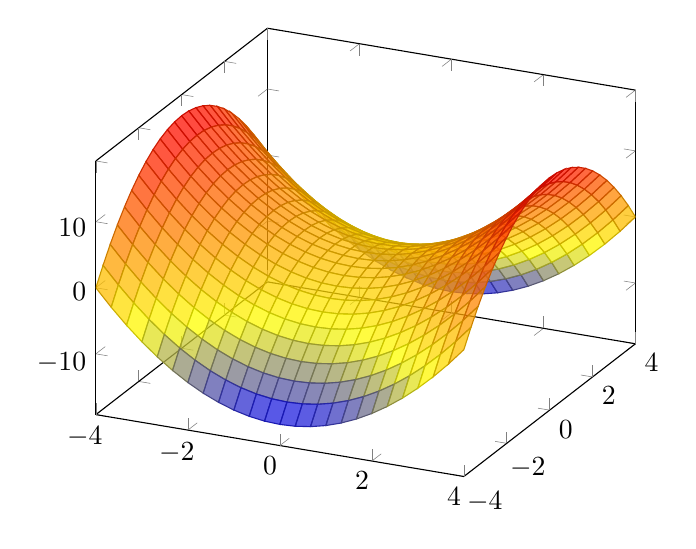
\begin{tikzpicture}
		\begin{axis}[view={25}{30},mark layer=like plot]
			\addplot3 [
				surf,
				shader=faceted,
				fill opacity=0.75,
				samples=25,
				domain=-4:4,
				y domain=-4:4,
				on layer=main,
			] {x^2-y^2};
		\end{axis}
	\end{tikzpicture}
	\caption{An example 3D plot done with PGFplots.}
\end{figure}

And, of course the code for generating the plot is given as follows:

<<<<<<< Updated upstream
\begin{code}{latex}
\begin{figure}[!ht]
  \centering
  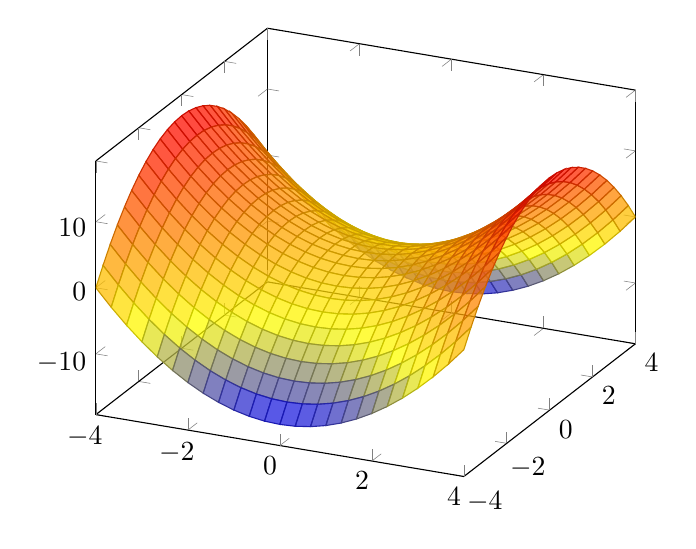
\begin{tikzpicture}
    \begin{axis}[view={25}{30},mark layer=like plot]
      \addplot3 [
      surf,
      shader=faceted,
      fill opacity=0.75,
      samples=25,
      domain=-4:4,
      y domain=-4:4,
      on layer=main,
      ] {x^2-y^2};
    \end{axis}
  \end{tikzpicture}
  \caption{An example 3D plot done with PGFplots.}
\end{figure}
\end{code}
=======
\begin{Code}{latex}{A 3D PGF plot}
	\begin{figure}[!ht]
		\centering
		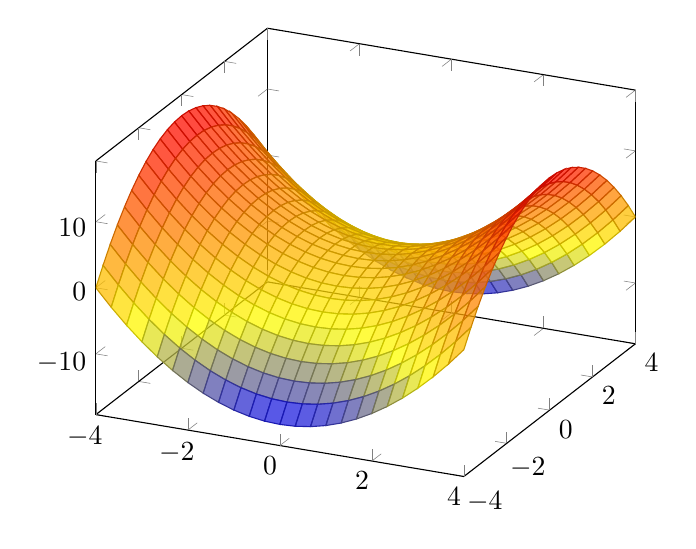
\begin{tikzpicture}
			\begin{axis}[view={25}{30},mark layer=like plot]
				\addplot3 [
					surf,
					shader=faceted,
					fill opacity=0.75,
					samples=25,
					domain=-4:4,
					y domain=-4:4,
					on layer=main,
				] {x^2-y^2};
			\end{axis}
		\end{tikzpicture}
		\caption{An example 3D plot done wit PGFplots.}
	\end{figure}
\end{Code}
>>>>>>> Stashed changes

Some options worth mentioning are as follows:

\begin{hgitemize}
	\item[\pcode{surf}] Generates a \hlight{surface} based on the 2D
	data it was given (in this case these are $x$ and $y$).
	\item[\pcode{shader}] Describes, basically how each segment should be
	filled.
	\item[\pcode{samples}] Similar to 2D plots, tells how many data points will
	be measured. However, make a note that 3D is significantly more taxing
	on the TeX memory than 2D and making this sampling high may result in
	exceeding the memory limit.
\end{hgitemize}

\end{document}

%%% Local Variables:
%%% coding: utf-8
%%% mode: latex
%%% TeX-command-extra-options: "-shell-escape"
%%% TeX-master: t
%%% TeX-engine: luatex
%%% End:

